\documentclass[conference,onecolumn]{IEEEtran}
\usepackage{amsmath,amssymb,amsfonts}
\usepackage[table,xcdraw]{xcolor}
\usepackage[spanish]{babelbib}
\usepackage[spanish]{babel}
\usepackage{algorithmic}
\usepackage{longtable}
\usepackage{setspace}
\usepackage{graphicx}
\usepackage{multirow}
\usepackage{textcomp}
\usepackage{graphicx}
\usepackage{pdfpages}
\usepackage{cite}
\usepackage{here}
\usepackage{url}

\IEEEoverridecommandlockouts
% \onehalfspacing

\ifCLASSINFOpdf
\else
\fi

\makeatletter
\newcommand{\linebreakand}{%
    \end{@IEEEauthorhalign}
    \hfill\mbox{}\par
    \mbox{}\hfill\begin{@IEEEauthorhalign}
}
\makeatother

\newcommand{\cen}{\centering}

\title{Diseño para un computador orientado hacia la visualización científica y realidad virtual tipo CAVE}

\author{
    \IEEEauthorblockN{1\textsuperscript{ro} Cristhian Díaz}
    \IEEEauthorblockA{\textit{Escuela de Ingeniería de Sistemas} \\
    \textit{Universidad Industrial de Santander}\\
    Bucaramanga, Colombia \\
    andresdiaz0608@gmail.com}
    \and

    \IEEEauthorblockN{2\textsuperscript{do} Diego Lozada}
    \IEEEauthorblockA{\textit{Escuela de Ingeniería de Sistemas} \\
    \textit{Universidad Industrial de Santander}\\
    Bucaramanga, Colombia \\
    lonidian@hotmail.com}

    \linebreakand
     
    \IEEEauthorblockN{3\textsuperscript{ro} Hendrik López}
    \IEEEauthorblockA{\textit{Escuela de Ingeniería de Sistemas} \\
    \textit{Universidad Industrial de Santander}\\
    Bucaramanga, Colombia \\
    hendriklop2106@hotmail.com}
    
    \and
    \IEEEauthorblockN{4\textsuperscript{to} Daniel Delgado}
    \IEEEauthorblockA{\textit{Escuela de Ingeniería de Sistemas} \\
    \textit{Universidad Industrial de Santander}\\
    Bucaramanga, Colombia \\
    danieldavid2001@gmail.com}
}

\def\BibTeX{{\rm B\kern-.05em{\sc i\kern-.025em b}\kern-.08em
    T\kern-.1667em\lower.7ex\hbox{E}\kern-.125emX}}
    
\begin{document}

\maketitle

\begin{abstract}
    La Visualización Computacional, se refiere al como, con el uso de computadores y diferentes herramientas de software, podemos transformar grandes cantidades de datos recolectados en diferentes elementos gráficos que permiten una mayor compresión de la información recopilada. Siendo así, se plantea la necesidad de una \textit{Spin-Off} universitaria la cual requiere de una solución computacional con el fin de realizar dichas visualizaciones manteniendo la capacidad para HPC y paralelismo respectivo. Para el desarrollo de la solución propuesta al problema planteado por la empresa, fue necesario tener en cuenta varios factores y condiciones a las cuales debíamos apegarnos para satisfacer la problemática planteada a partir de la identificación de los componentes adecuados, y la cotización de los mismos. Tras la selección de todos los componentes, tenemos como resultado la configuración final de nuestro sistema. Es de esperarse que el equipo propuesto pueda realizar, a satisfacción, la ejecución de los diferentes procesos y aplicaciones requeridos por la empresa.
\end{abstract}

{
    \begin{center}
        \textbf{\small Abstract}
    \end{center}
    \hspace*{0.7cm} 
    \small
    Computational Visualization refers to how, with the use of computers and different software tools, we can transform large amounts of data collected into different graphic elements that allow a greater compression of the information collected. This being the case, a university Spin-Off requires a computational solution in order to carry out said visualizations while maintaining the capacity for HPC and respective parallelism. For the development of the proposed solution to the problem posed by the company, it was necessary to take into account several factors and conditions to which we had to adhere to satisfy the problems raised from the identification of the appropriate components, and the quotation of them. After the selection of all the components, we have as a result the final configuration of our system. It is expected that the proposed team can carry out to satisfaction the execution of the different processes and applications required by the company.
}

\begin{IEEEkeywords}
    \centering
    Arquitectura de computadores, Diseño computacional, High Performance Computing, Parallel Processing, CUDA
\end{IEEEkeywords}

\section{Introducción}
En las ciencias de la computación, la Visualización se refiere al como, con el uso de computadores y diferentes herramientas de software, podemos transformar grandes cantidades de datos recolectados en diferentes elementos gráficos que permiten una mayor compresión de la información recopilada \cite[Pág. 150]{vis}. Es gracias a la Visualización Computacional, por la cual el realizar análisis de los datos recolectados en simulaciones, o a partir de sensores, se convierten en tareas considerablemente más sencillas que el tratar de encontrar patrones y tendencia en cientos de mediciones y cifras replegadas en una hoja de cálculo. Dentro de la visualización, hay multiples ramas las cuales poseen diferentes enfoques y aplicaciones específicas dependiendo de lo que se requiera realizar al igual que el origen de los datos a trabajar. Una de estas ramas, y la más relevante para el presente documento, es la rama de la visualización científica (SciVis). En esta, el enfoque está principalmente orientado a la visualización de fenómenos tridimensionales, que competen a la medicina, meteorología, biología, el sector energético, entre otros \cite{SciVis}. En consecuencia, al ser la visualización científica una de las herramientas más importantes en cuanto al tratamiento de datos, existe una alta demanda por este tipo de servicios al igual que los equipos necesarios para llevarse a cabo. \medbreak 

Uno de estos casos es el que compete al presente documento. Se plantea el caso de una empresa pequeña, similar a una \textit{Spin-Off} universitaria, la cual realiza el desarrollo de aplicaciones para visualización científica orientadas principalmente al sector energético de \textit{Oil and Gas}. Debido a esto, esta organización requiere de una solución para poder realizar diferentes tipos de visualizaciones inmersivas con el uso de tecnología de Realidad Virtual (VR) tipo CAVE (\textit{Cave automatic virtual environment}). De igual manera, es de resaltar que los desarrollos están siendo realizados con diferentes lenguajes de programación, tales como C/C++, CUDA, JAVA, Python y R; directivas, OpenACC, OpenCL, Matlab; las librerias, OpenGL y OpenCV; al igual que compiladores, ambientes de desarrollo y ejecución conocidos. De igual manera, dentro de estos requerimientos iniciales, se plantea la necesidad de soportar computación de alto rendimiento (HPC) y paralelismo al igual que la posibilidad de tener una alta calidad gráfica sin despreciar las aplicaciones en CUDA; asimismo se necesita una capacidad de red considerable debido a las conexiones hacia una red privada y una académica.
\cite{arqCom}  \medbreak

Partiendo de esto, en el presente documento se realizará el diseño, al igual que la cotización, de una posible solución a la problemática a la que esta empresa se enfrenta. Esto se realizará a partir del planteamiento de un equipo computacional cuyos componentes, seleccionados a partir de las especificaciones y características individuales de cada una de las partes, teniendo en cuenta la limitación del presupuesto dado; permitan el correcto desarrollo de las actividades de la empresa. \medbreak 

\section{Objetivos}
\subsection{Objetivo General}
\begin{itemize}
    \item Diseñar un sistema de computo que permita a la empresa la visualización de la ejecución de procesos de visualización científica en un ambiente de realidad virtual tipo CAVE. \medbreak
\end{itemize}

\subsection{Objetivos Específicos}
\begin{itemize}
    \item Definir los requerimientos que se adapten de mejor manera a la problemática.presentada por la empresa \medbreak
    \item Identificar los componentes que cumplan con los requerimientos establecidos.\medbreak
\end{itemize}

\section{Metodología}
Para el desarrollo de la solución propuesta al problema planteado por la empresa, fue necesario tener en cuenta varios factores y condiciones a las cuales debíamos apegarnos para satisfacer la problemática planteada. En este sentido, se realizó el desarrollo en 3 partes. La determinación de los requerimientos, la identificación de los componentes adecuados, y la cotización de los mismos.

Siendo así, se inicio con la determinación de los requerimientos del sistema en cuestión. Estos han sido propuestos de manera genérica con el fin de dar cabida a la comparación de multiples componentes mientras se cumplen las expectativas del sistema. Estas se presentan en el cuadro \ref{tab:ReqTable}.

\begin{longtable}[c]{|c|l|c|}
    \hline
    \rowcolor[HTML]{9B9B9B} 
    Categoría &
      \multicolumn{1}{c|}{\cellcolor[HTML]{9B9B9B}Descripción} &
      Requisitos \\ \hline
    \endfirsthead
    %
    \endhead
    %
    GPU &
      \begin{tabular}[c]{@{}l@{}}Partiendo de que la principal necesidad de la empresa, \\ que es la realización de visualización científica, es \\ menester una gran capacidad de procesamiento gráfico. \\ Adicionalmente, es necesario, especialmente por el énfasis \\ en procesamiento en paralelo, una gran disponibilidad de \\ núcleos CUDA que permita la ejecución de este tipo de \\ aplicaciones.\end{tabular} &
      \begin{tabular}[c]{@{}c@{}}Gran capacidad de VRAM.\\ Gran cantidad de CUDA cores.\\ Alto ancho de banda de memoria.\end{tabular} \\ \hline
    CPU &
      \begin{tabular}[c]{@{}l@{}}La principal característica de nuestra CPU a escoger, sea \\ capaz de soportar la solución gráfica que vayamos a escoger. \\ Es decir, es necesario que la cantidad de lanes debe ser\\ suficiente para abarcar la cantidad de GPUs empleadas. En \\ igual medida, es de interés, especialmente para HPC, una \\ alta cantidad de cores y threads que permitan una facilidad \\ en la ejecución de las diferentes aplicaciones.\end{tabular} &
      \begin{tabular}[c]{@{}c@{}}Multiples Cores y Threads.\\ Gran cantidad de PCI Lanes.\\ Alta capacidad de cache.\\ TDP relativamente bajo.\\ Alta frecuencia de operación.\\ Configuración 2P.\end{tabular} \\ \hline
    RAM &
      \begin{tabular}[c]{@{}l@{}}El caso de la memoria existen no existen realmente \\ condiciones especiales. En este caso los factores \\ discriminantes están dados por la máxima cantidad que \\ soporte la CPU seleccionada y a la mayor velocidad disponible. \\ De manera ideal, la cantidad de módulos debe ser suficiente \\ para poder llenar los canales disponibles con el fin de \\ aprovechar los beneficios que viene de emplearlos en su \\ totalidad.\end{tabular} &
      \begin{tabular}[c]{@{}c@{}}Memoria registrada.\\ Alta frecuencia de operación.\\ Alta densidad de memoria.\end{tabular} \\ \hline
     Red &
      \begin{tabular}[c]{@{}l@{}}Las capacidades de red de la máquina tienen que se suficientes \\ para poder realizar operaciones dentro de la red tanto privada \\ como académica. Es por esto que se espera que se tengan las \\ capacidades de red necesarias para realizar estas operaciones.\end{tabular} &
      \begin{tabular}[c]{@{}c@{}}Capacidad para 10 Gigabit\\ Ethernet.\\ Soporte para conexiones \\ RJ45 y SFP+.\end{tabular} \\ \hline
    Almacenamiento &
      \begin{tabular}[c]{@{}l@{}}El almacenamiento, debido a la configuración que estamos\\ manejando, realmente no cae dentro de las principales \\ preocupaciones puesto que gran parte de la información será \\ manejada en red. En este sentido, sólo se tiene pensado en \\ priorizar el disco de arranque al igual que el almacenamiento \\ necesario para la configuración y las aplicaciones del dispositivo.\end{tabular} &
      \begin{tabular}[c]{@{}c@{}}Alta velocidad read/write\\ Capacidad media.\end{tabular} \\ \hline
    Barebones\footnote{Barebones se refiere a los componentes del chasis, la tarjeta madre y las PSU que serán empleadas para el sistema. \cite{barebones}} &
      \begin{tabular}[c]{@{}l@{}}El principal enfoque de debe tener el barebones está en la \\ capacidad de integrar todos los componentes seleccionados. \\ De igual manera, es necesario que se pueda surtir de poder a \\ todos los elementos para la correcta operación de los mismos.\end{tabular} &
      \begin{tabular}[c]{@{}c@{}}PSU redundantes.\\ Compatibilidad con el procesador \\ y la solución gráfica seleccionada.\\ Suficientes puertos para RAM y\\ PCIe. \\ GPU oriented.\end{tabular} \\ \hline
    \caption{Descripción de los requisitos del sistema}
    \label{tab:ReqTable}\\
\end{longtable}

A partir de lo realizado en la primera parte, se empezó así la selección de algunas de las partes que cumplen con las características establecidas para el sistema en cuestión. Seguidamente, se realizaron las comparaciones respectivas entre cada una de las partes para así determinar cual era la parte más adecuada en términos tanto de rendimiento como presupuesto. \medbreak 


\section{Desarrollo}
Partiendo de las características establecidas de manera inicial respecto a las necesidades de la empresa en cuestión, se realizó la selección general de cada uno de los componentes que cumplían las condiciones establecidas. A partir de esta selección, se realizó la evaluación de cada uno de los elementos para poder determinar cuales serían los indicados que cumplieran con los requerimientos de la organización. 

\subsection{GPU: NVIDIA GPU Accelerator}
Como ya se ha establecido en varios momentos a lo largo del presente documento, uno de las principales necesidades de la empresa está en adquirir una solución gráfica considerable para la correcta realización de sus aplicaciones de visualización científica al igual que la capacidad en términos de paralelismo y HPC. Siendo así, y aunque las características presentadas por AMD y sus GPU Accelerator MI100 son bastante interesantes, especialmente debido a sus declaraciones en cuanto a sus capacidades de procesamiento \cite{amdMI100}; es la necesidad de aplicaciones CUDA las cuales nos hacen decantarnos por una solución dentro de las familias de NVIDIA. \cite{CUDAnt}  \medbreak

Ampere es la más reciente microarquitectura de NVIDIA destacada por características como NVLink 3.0, la tercera generación de Tensor Cores, el cambio a la interfaz de PCI Express 4.0 y muchas otras exclusivas a su tarjeta de más alta gama (A100) como MIG, CUDA Compute Capability 8.0, HBM2 y, por supuesto, el proceso 7 nm FinFET de TSMC \cite{nvidiaAmpBlog}. Esta familia también se divide en 3 series: Geforce 30 series, Workstation GPUs (la antes denominada Quadro) y Data Center GPUs (antes denominada Tesla). La 30 series es la dedicada a consumidores (particularmente gamers) y cuenta con RT Cores de segunda generación adicionales a los Tensor Cores de tercera presentes en las demás tarjetas \cite{nvidia30}; las Data Center GPUs están diseñadas para configuraciones en servidores y/o para usos de visualización, simulación e inteligencia artificial y cuentan con extremas cantidades de memoria, CUDA Cores y Tensor Cores; y las Workstation GPUs son un punto en la mitad creado para situaciones donde se necesitan realizar los procesos mencionados en las Data Center GPUs, pero también se requiere fácil acceso a RT Cores de segunda generación como en las 30 series \cite{nvidiaAmp}. Debido a las necesidades del cliente se deben revisar opciones dentro de la gama para Data Centers. \medbreak

Entre esta las dos tarjetas a destacar serían la A40 y la A100 (40GB). Las A100 gozan de 40GB de memoria HBM2, 6912 CUDA Cores y una banda ancha de 1.6 TB/s; volviéndola una excelente elección para entrenamiento de inteligencia artificial y redes neuronales \cite{pny}. Por otra parte, las A40 cuentan con 48GB de memoria GDDR6 ECC, 10752 CUDA Cores y 696 GB/s de banda ancha; permitiéndole especializarse en renderización y rendimiento gráfico sin sacrificar una elevada capacidad para entrenamiento de inteligencia artificial comparada con la RTX 6000 de la generación Turing \cite{nvidiaa40}. Tomando en cuenta lo anterior, se hicieron cotizaciones en las que se buscó comparar el rendimiento de una configuración con A100s ante otra con A40s intentando mantener el precio lo más cercano posible. De esta manera se llegó a una opción A con 4 A100s de 40GB y una opción B con 8 A40s; siendo la segunda tan solo aproximádamente dos mil dólares más costosa. \medbreak

Debido a su mayor cantidad de CUDA Cores, mayor memoria y menor precio, se decide optar por la opción B. Los recursos añadidos de 8 A40s conectadas con NVLink 3.0 superan los que se obtendrían con 4 A100s por una diferencia de precio relativamente mínima, permitiendo maximizar la cantidad y el rendimiento de simulaciones y visualizaciones científicas simultáneas.


\subsection{CPU: Team Blue vs Team Red}
Comercialmente hablando, el mercado de los procesadores está dividido mayoritariamente, y especialmente en cuanto a soluciones tipo \textit{data center} se refiere; en dos compañías principales, Intel y AMD. Lo primero a considerar sería la opción de Intel y su familia de procesadores Xeon Platinum Scalable la cual está orientada, principalmente, hacia operaciones de HPC al igual que otras aplicaciones de \textit{data center}. Estos procesadores de Intel, en consecuencia, hacen parte de los posibles componentes que se adapten los requerimientos establecidos gracias a la gran flexibilidad que esta familia tiene consigo, dandonos opciones desde 8 a 40 núcleos al igual que un cache considerable junto con un rango de 150 a 270 W de TPD. \cite{intelPlat, intelXeonHPC, intelXeon} \medbreak 
  
En el caso de AMD, la tercera generación de procesadores Epyc (Epyc 7003), la cual, al igual que Intel, está enfocada a las soluciones para servidores en las cuales las operaciones de HPC y aplicaciones similares también es necesario \cite{AMDHPC}. En simultaneo, se tiene un mayor rango entre 8 a 64 núcleos, aunque con TPDs más consistentes (180 - 280 W) (Ver figura \ref{fig:amdData}). \medbreak

Hasta el momento, las comparaciones generales entre las 2 familias de procesadores se ve relativamente cercana en cuanto a las características presentadas hasta el momento se refiere. Sin embargo, una de las principales limitaciones que presenta la familia Xeon, es la relativa baja disponibilidad de lanes de PCIe de tercera generación, de 48 a 64; a las cuales nuestra solución gráfica debe adaptarse si lo comparamos con las 128 lanes de PCIe de cuarta generación que nos presenta la familia Epyc. Entonces, es por este factor diferenciador, el cual nos permite trabajar sin limitaciones en cuanto a la cantidad de tarjetas A40 se empleen. Entonces, partiendo de la clara ventaja que presentan los procesadores de Epyc, especialmente en las condiciones en las cuales nos encontramos; habría que determinar la configuración y referencia especifica para nuestro sistema. \medbreak

\begin{figure}
  \centering
  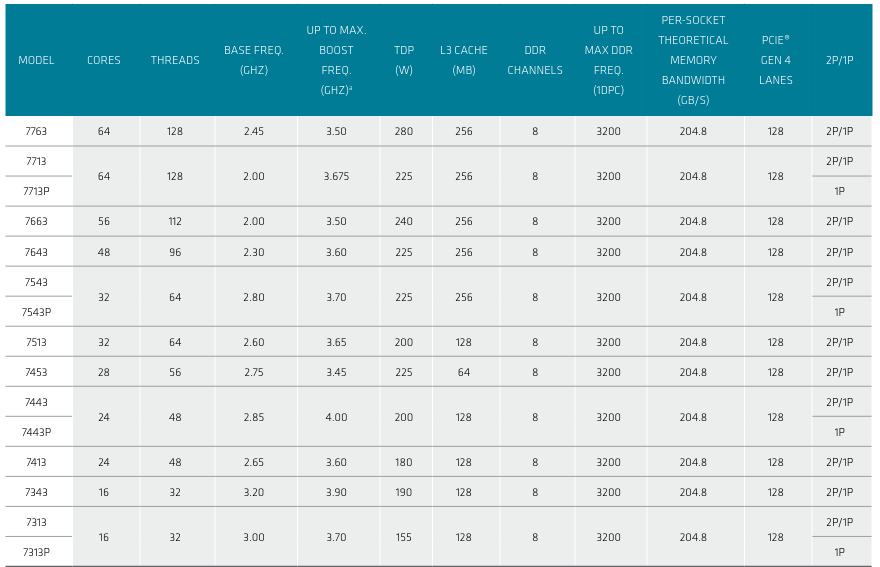
\includegraphics[scale=0.5]{AMD.png}
  \caption{Datasheet de Epyc Milán. \cite{AMDdatasheet}}
  \label{fig:amdData}
\end{figure}

Partiendo de la selección de un procesador de la serie Epyc 7003, ha de ser considerado cuales de estos poseen capacidad de ser usados en una configuración de 2 sockets la cual es imperativa para acceder a las capacidades de paralelismo \cite{techtarget_2019}. Sin embargo, gracias a que las características generales de esta familia de procesadores es considerable y a la presencia de un presupuesto limitado para la solución, nuestras opciones están determinadas, principalmente, la mejor relación precio-rendimiento. En este caso, y considerando las limitaciones presupuestales, la opción que mejor se adapta sería el procesador Epyc 7513. \medbreak  

\subsection{Barebones, RAM y Almacenamiento}
Teniendo claras los componentes principales que cumplen con las necesidades computacionales de la empresa, es posible realizar la selección de la RAM, el almacenamiento y barebones que harán parte de la solución. \medbreak

Lo primero a considerar está en el tipo de barebones que se empleará. Conociendo el uso que se le dará a la solución, es claro que el barebones deberá ser \textit{GPU oriented} en tanto se requiere un número considerable de procesadores gráficos al igual que el soporte de multiples CPUs. Seguidamente, y debido a estas condiciones, lo más apropiado, especialmente para la simplificación de la logistica al igual que la conveniencia de tratar únicamente con una sola entidad, sería el usar un proveedor. \medbreak

En este caso, nos decantaremos por Thinkmate, un proveedor de Estados Unidos; el cual nos presenta con múltiples opciones (Ver figura \ref{fig:thinkmate}) en cuanto a servidores orientados a la visualización y HPC \cite{thinkmate}. De manera inicial, nos presenta varias opciones de las cuales, en este caso, tendremos que descartar algunas por terminos de presupuesto. \medbreak

\begin{figure}[h!]
  \cen
  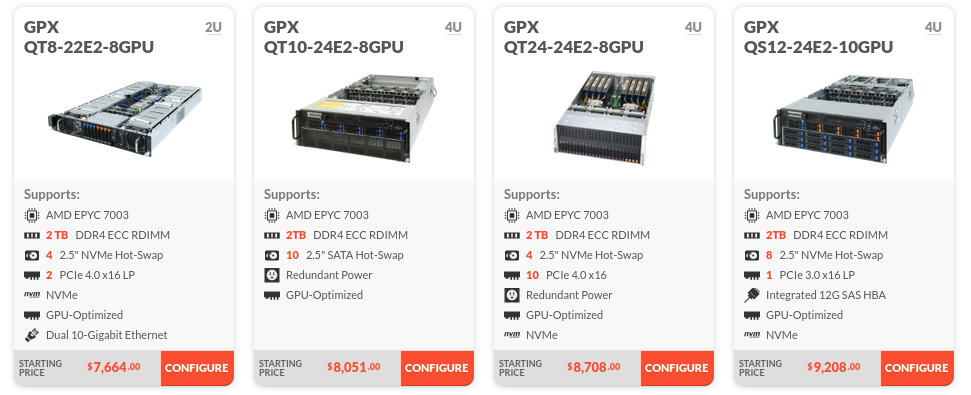
\includegraphics[scale=0.5]{think.png}
  \caption{Opciones presentadas por Thinkmate \cite{thinkmate}}
  \label{fig:thinkmate}
\end{figure}

Explorando de manera general, podemos ver que, para el barebones GPX QT24-24E2-8GPU, dentro de las características más relevantes, es el hecho de que posee 10 puertos PCIe4.0x16, a diferencia de las otras unidad con menos puertos o de generaciones anteriores. Esto es especialmente relevante por la configuración que buscamos para nuestra solución gráfica la cual, de ser instalada en esta unidad, podría ser aprovechada casi que en su totalidad sin problema alguno. En consecuencia, gracias a lo anteriormente descrito,  al igual que características de poder redundante al igual que una alta capacidad de memoria RAM, será esta la opción que emplearemos dentro del equipo final. \medbreak

Explorando un poco más las opciones que nos presenta Thinkmate para la configuración de su GPX QT24-24E2-8GPU, en términos de memoria RAM están varias configuraciones posibles. En este caso, siguiendo los lineamientos establecidos durante la metodología, se acomodarán 32 módulos de RAM ECC DDR4 a 3200 MHz registrada de la mayor capacidad posible para cada uno de los 64 núcleos de la configuración 2P a trabajar. Teniendo en cuenta las limitaciones de presupuesto, la máxima capacidad posible, siguiendo los precios dados por Thinkmate, nos dejan con la opción de 32 módulos de 32 Gb con las características indicadas, para un total de 1 Tb de RAM. \medbreak

Así mismo, se nos presentan varias opciones en cuanto a almacenamiento se refiere, sin embargo, como ya hemos establecido, una gran cantidad de espacio no es una de las prioridades. En consecuencia, sólo se tendrá en consideración el boot drive en una capacidad media, que en este caso, sería un SSD NVMe de 1 Tb. 

\subsection{Red: Conexión 10-Gigabit}
En el caso de conexiones a red, más allá de la información relacionada con las conexiones hacia las redes tanto académicas como privadas, no tenemos mucha información al respecto. Por ello, nuestro enfoque está más al tener el mínimo comercial de 10GbE (10 Gigabit Ethernet), al igual que conexiones por cable categoría 5 al igual que conexiones SFP+. \medbreak

En consecuencia, como solución, se tuvo en consideración el uso de 2 tarjetas de red, Ethernet Network Adapter X710-T2L y X710-DA2, las cuales permitieran, cada una de ellas, un tipo de conexión diferente; esto así con el fin de abarcar todas las posibilidades en cuanto a la configuración interna de las redes se refiere. Sin embargo, se ha de resaltar que esta selección, más allá de la capacidad de 10GbE de las tarjetas, es considerada arbitraria al igual que bastante flexible en el caso de no necesitar uno de los tipos de conexiones.

\subsection{Conceptos misceláneos}
Al igual que los componentes de la solución, se tuvieron en consideración algunos de los conceptos tales como los costos de envio e importación del equipo planteado. Esto debido a los efectos dentro del presupuesto que estos implican. \medbreak

El primero de estos conceptos, se refiere a los impuestos que se aplicarían en términos de la importación del equipo. Tomando a Colombia como nuestro ejemplo, los impuestos aplicados en términos de aranceles e impuesto al consumo, en este caso IVA; para el año 2021 sería del 10\% \cite{mincit} y 19\%\cite{rci} respectivamente, dando como resultado un total de impuestos del 29\% sobre el precio del equipo en cuestión.

En cuanto al envío se refiere, y aprovechando las ventajas logisticas de usar un proveedor como Thinkmate, es posible realizar la cotización del envío directamente. Para nuestra configuración seleccionada, se nos presenta la opción de 2 tipos de envio con la compañía FedEx. La primera, FedEx International Economy, con un valor de \$2,609.{\small00}; y FedEx International Priority, con un valor de \$3.664.{\small00} \cite{thinkmateHP}. Se ha de resaltar el que, aunque ambas opciones son viales, para el propósito de este ejercicio, se tomará el menor valor.


\section{Resultados}
Tras la selección de todos los componentes, tenemos como resultado la configuración final de nuestro sistema. Al haber cumplido con las características establecidas, es de esperarse que el equipo propuesto pueda realizar, a satisfacción, la ejecución de los diferentes procesos y aplicaciones requeridos por la empresa en términos de tanto HPC al igual que paralelismo dandole un enfoque a la calidad gráfica. De igual manera, teniendo en cuenta la configuración dada, se espera que el equipo no requiera una verdadera actualización de sus componentes en los próximos de 3 a 5 años. \medbreak

Siendo así, el resultado final del desarrollo es la configuración junto con los precios dados por Thinkmate al momento de la realización del presente documento (Ver anexo al final del documento\footnote{La configuración, vista desde la página de Thinkmate puede ser accedida con el código 533089 \cite{thinkmateConf}}). \medbreak

En cuanto al valor total presupuestado, tomando el valor dado por thinkmate, tanto como por el equipo, \$64,139.{\small00} \cite{thinkmateConf}; como el envio del mismo \$2,609.{\small00} \cite{thinkmateHP}; nos da un total de \$66,748.{\small00}. Teniendo en cuenta el valor considerado para los impuestos sobre el valor del equipo, nos daría el total de \$85,348.{\small31}. 

\section{Limitaciones}
Las limitaciones de la solución planteada se extienden, principalmente, al desconocimiento de algunas de las condiciones en las cuales va a ser operado el equipo. En consecuencia, gracias a estas ambiguedades, se nos presentan situaciones como la de la necesidad de cubrir ambos tipos de conectores en cuanto a red se refiere. En igual medida, el desconocimiento de la ubicación en la que será operada, no nos permiten realizar valoraciones en cuanto a la adaptabilidad del espacio se refiere u otras condiciones operativas. \medbreak

Así mismo, se tuvieron algunos problemas en cuanto a la recopilación de información en términos de \textit{benchmarks} de la gran mayoría de los componentes. Esto, derivado principalmente, del nicho en el cual estamos operando en términos de la accesibilidad de las piezas. Siendo así, gran parte de la información con la que se trabajó viene directamente de las mismas compañías que proveen los componentes. Aunque esto no evitó la selección de los componentes, sí nubló las estadísticas en cuanto al rendimiento dentro de un ambiente práctico.

\section{Conclusiones}
Tras la realización del presente documento, al igual que el desarrollo de su componente práctico, es posible contemplar el cumplimiento de los objetivos establecidos. Se considera que, al menos de manera teórica, fue posible realizar el diseño de una solución para la problemática presentada para la organización en cuestión respetando las limitaciones de presupuesto dadas. De igual manera, la realización del mismo, permitió un mayor entendimiento y acercamiento a las diferentes arquitecturas, especialmente en el marco de las GPUs. En igual medida, se reconocen las limitaciones del mismo en cuanto a su desarrollo y ejecución.


\bibliographystyle{IEEEtran}
\bibliography{ref}

{
    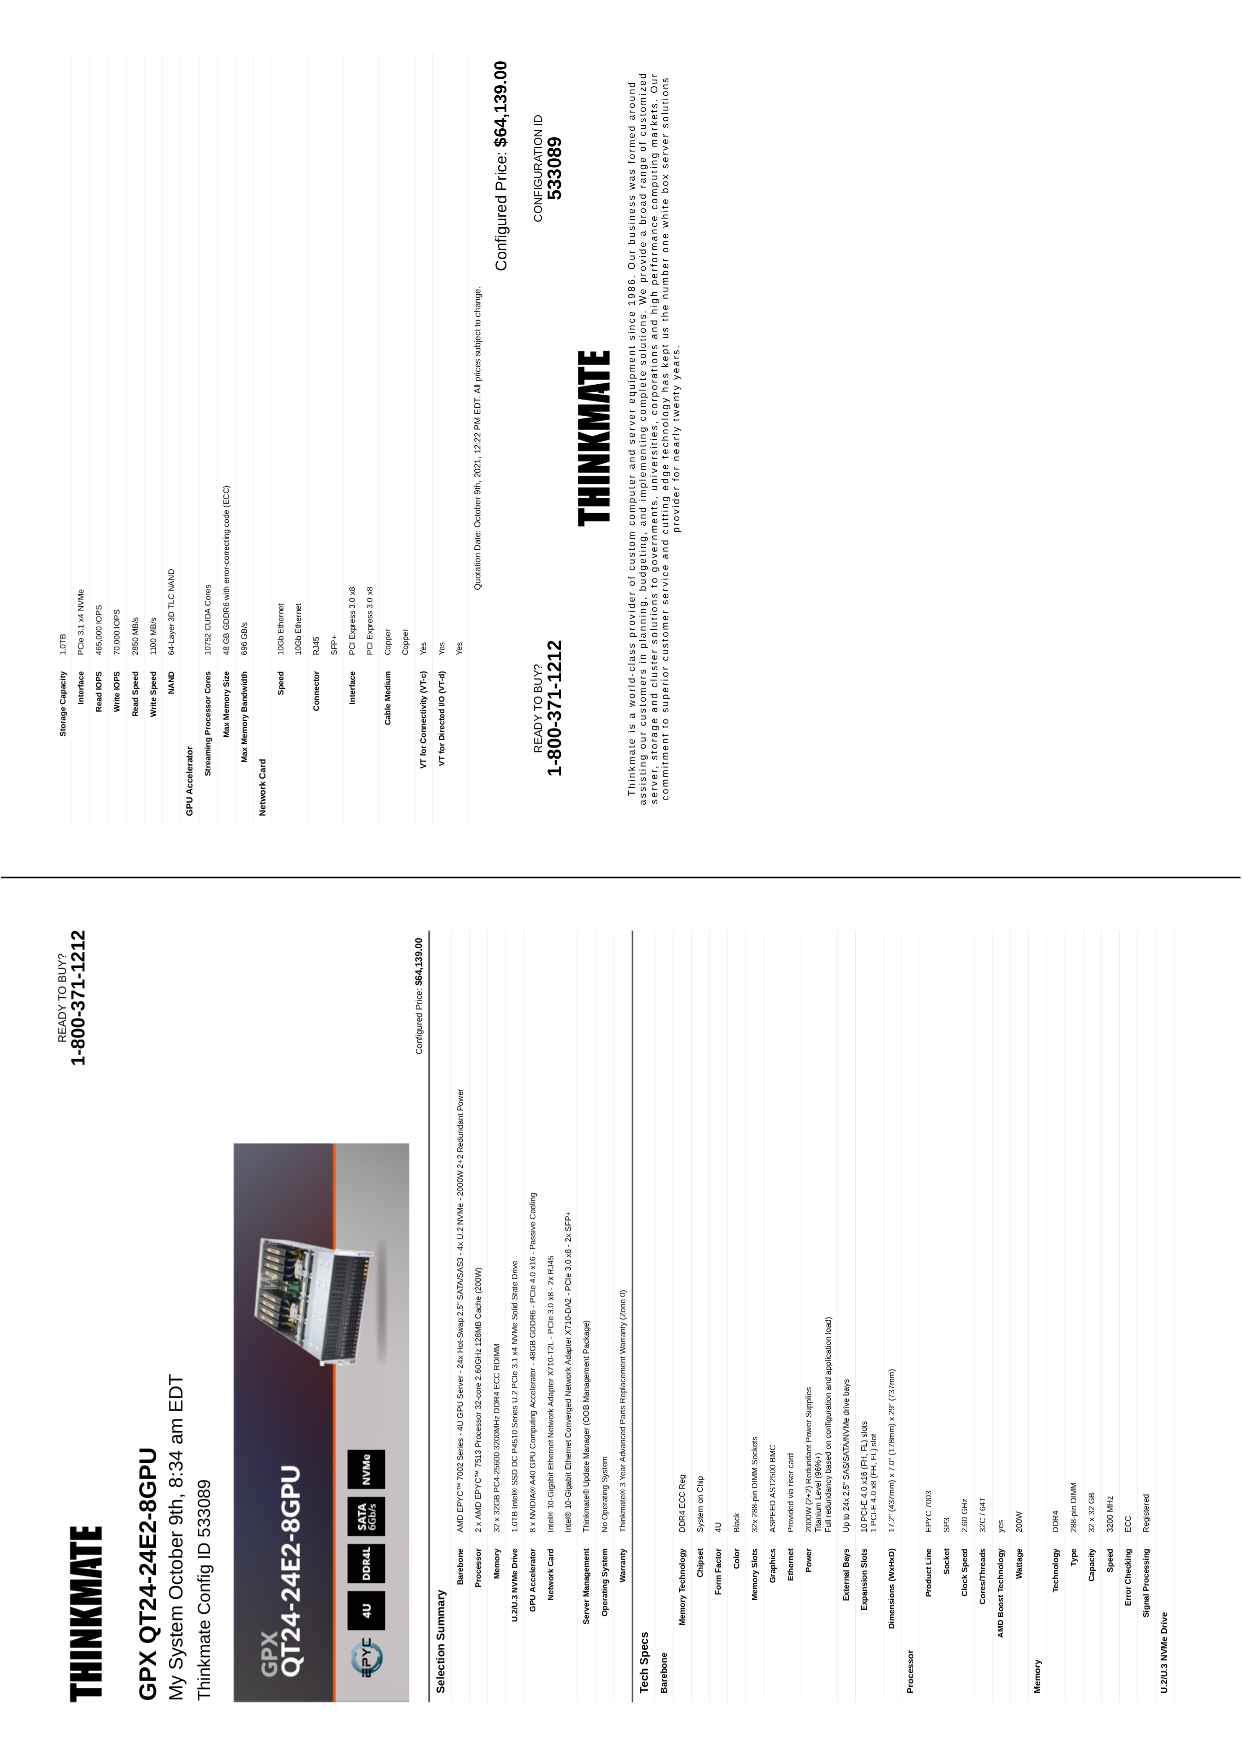
\includepdf[pages=1, landscape=false]{533089}
    \label{insert:cot}
}

\end{document}
